%!TEX root = ../SciVis.tex

The isolines can be visualised by selecting the option \emph{Isolines} from the \emph{Options} panel and they can be parameterised from the \emph{Contouring} panel. There are two kinds of isoline visualisations. First, the user can visualise isolines which corresponds to one particular scalar value which can be set and it is the \emph{Density rho}. In order to colorise the isolines the \emph{Colorise} option must be selected. The isoline visualisation has been implemented using the \emph{marching squares} method. We can directly compute the isolines of the density scalar dataset as its continuity is $C^1$. 

% implementation

Figure~\ref{fig:isoline} depicts the isoline visualisation which corresponds to the scalar density value $rho = 0.5$. Figure~\ref{fig:isoline}(a) shows only the colorised isoline, while in Figure~\ref{fig:isoline}(b) we decided to visualise the isoline together with the smoke field but not to colorise the isoline. This provides a clearer overview of the total range of scalar values and to which scalar value do the isolines correspond.

\begin{figure}[htbp]
\begin{center}
\begin{minipage}[t]{0.48\textwidth}
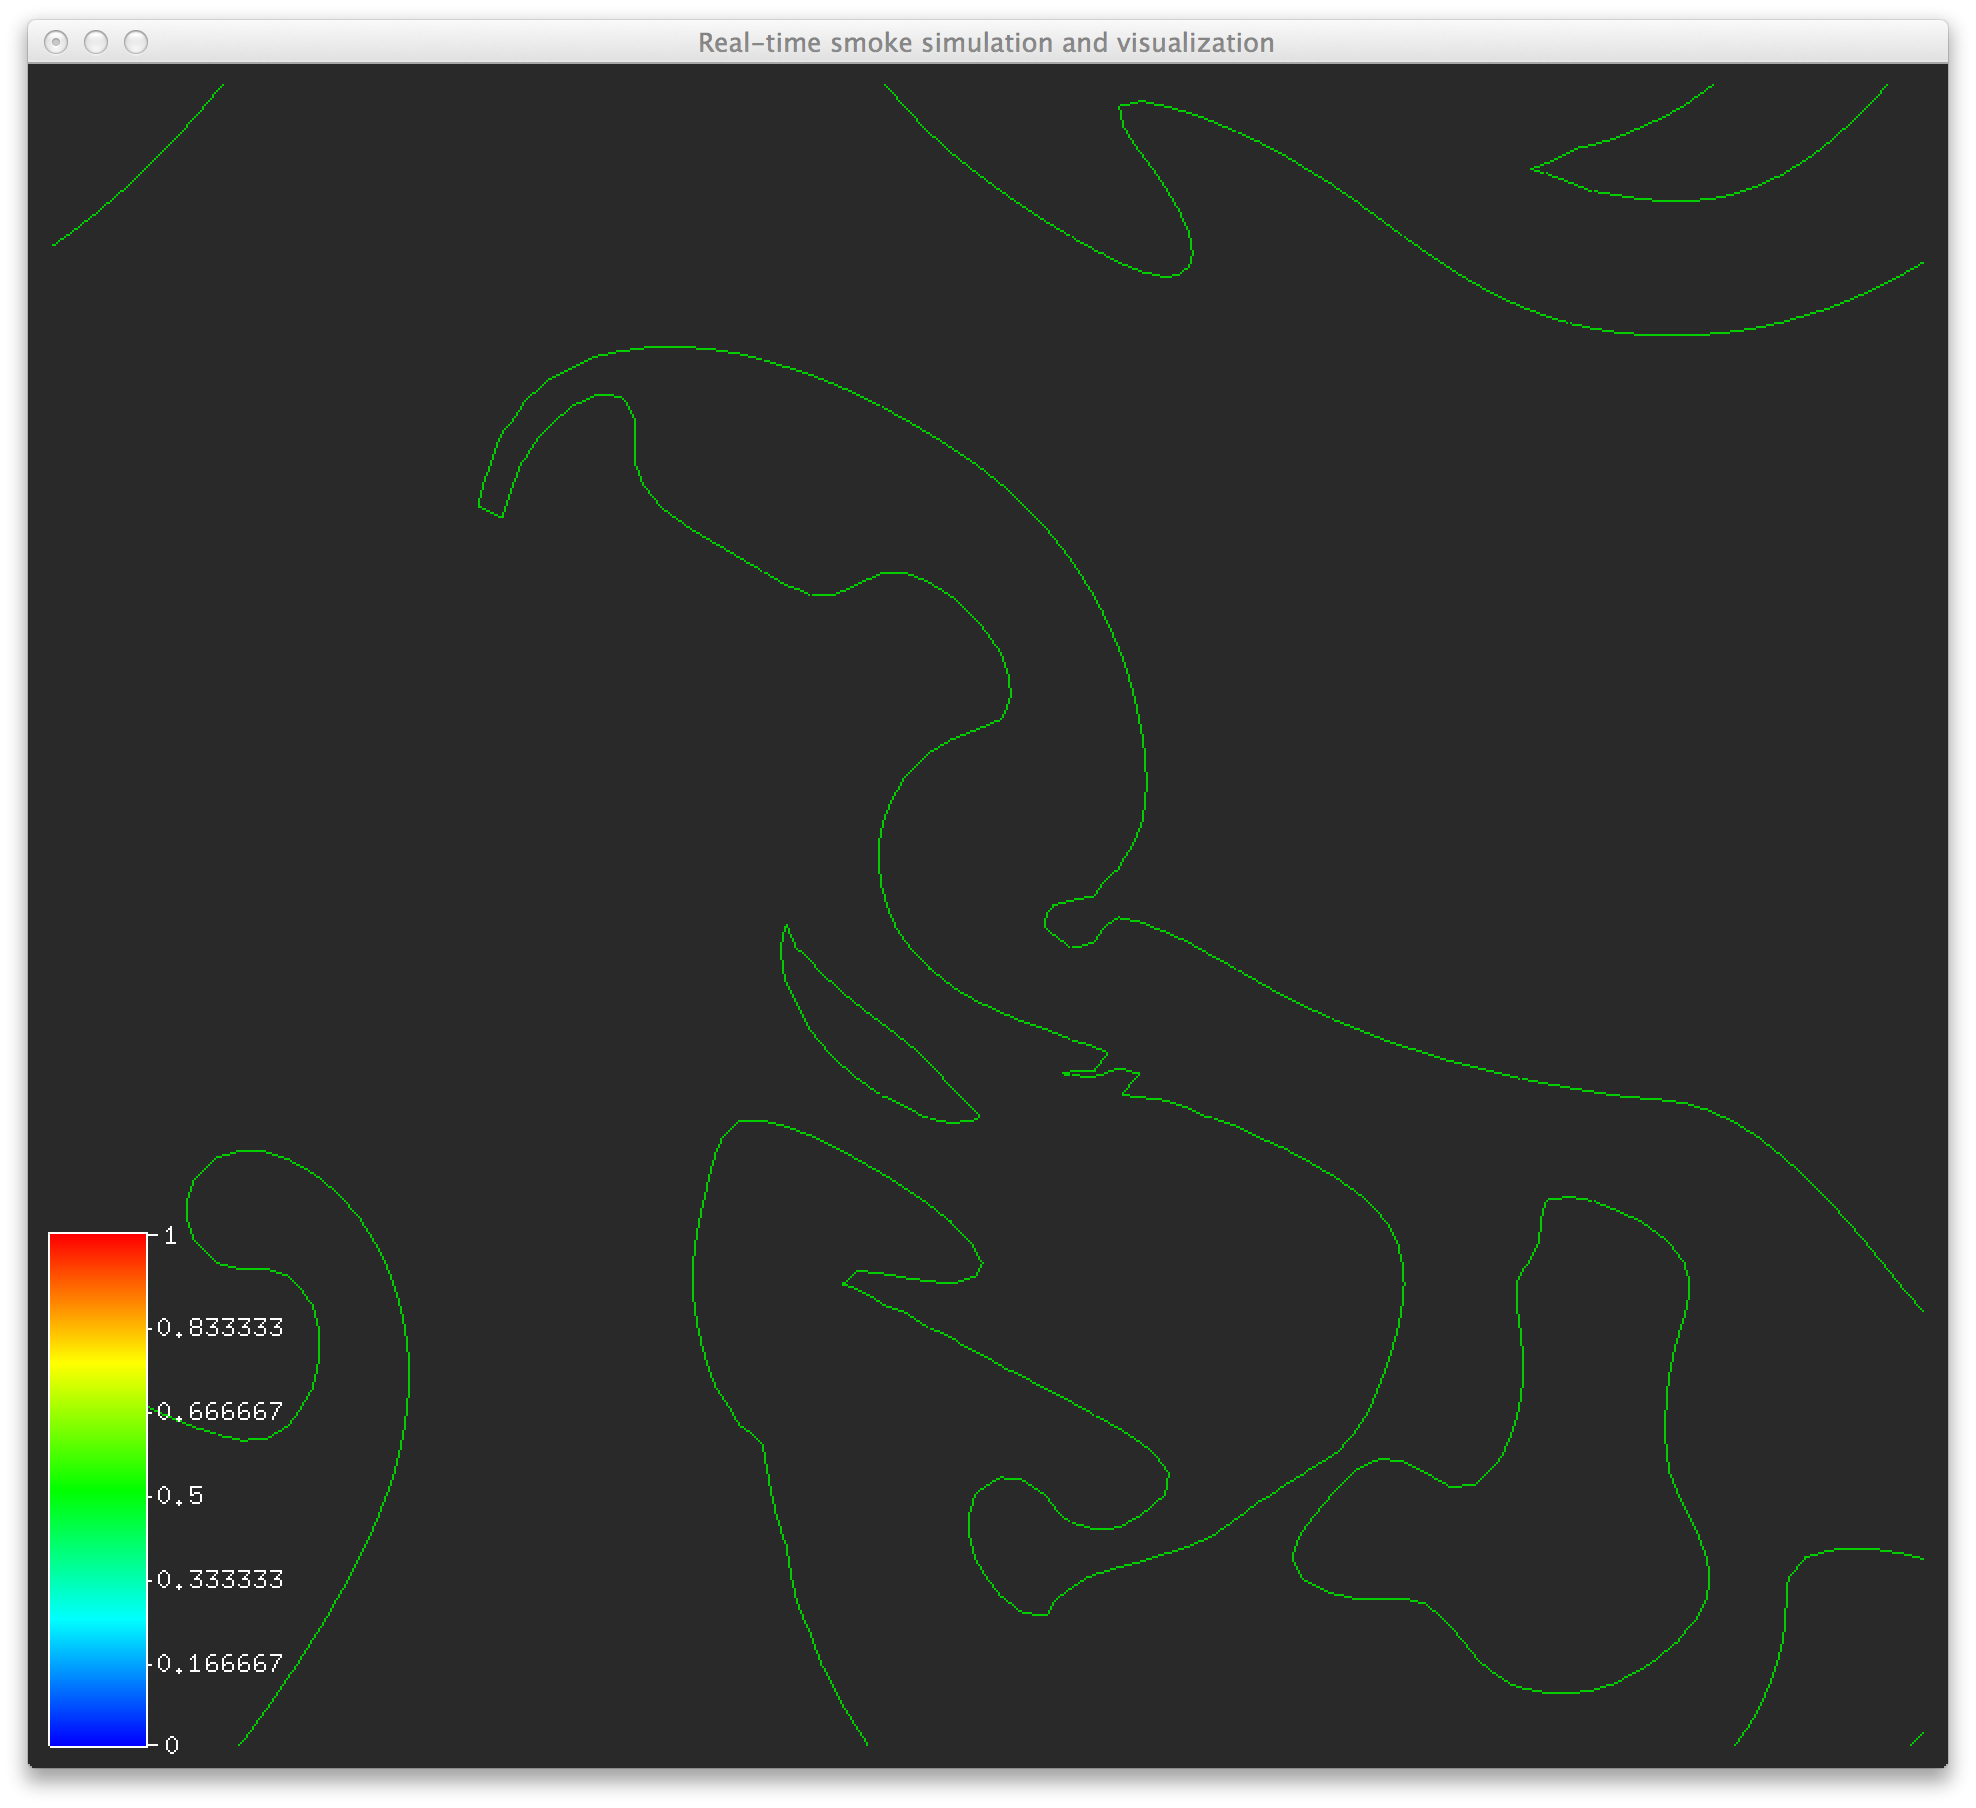
\includegraphics[height=2.7in]{figures/isolines/isoline.png}
\end{minipage}
\begin{minipage}[t]{0.48\textwidth}
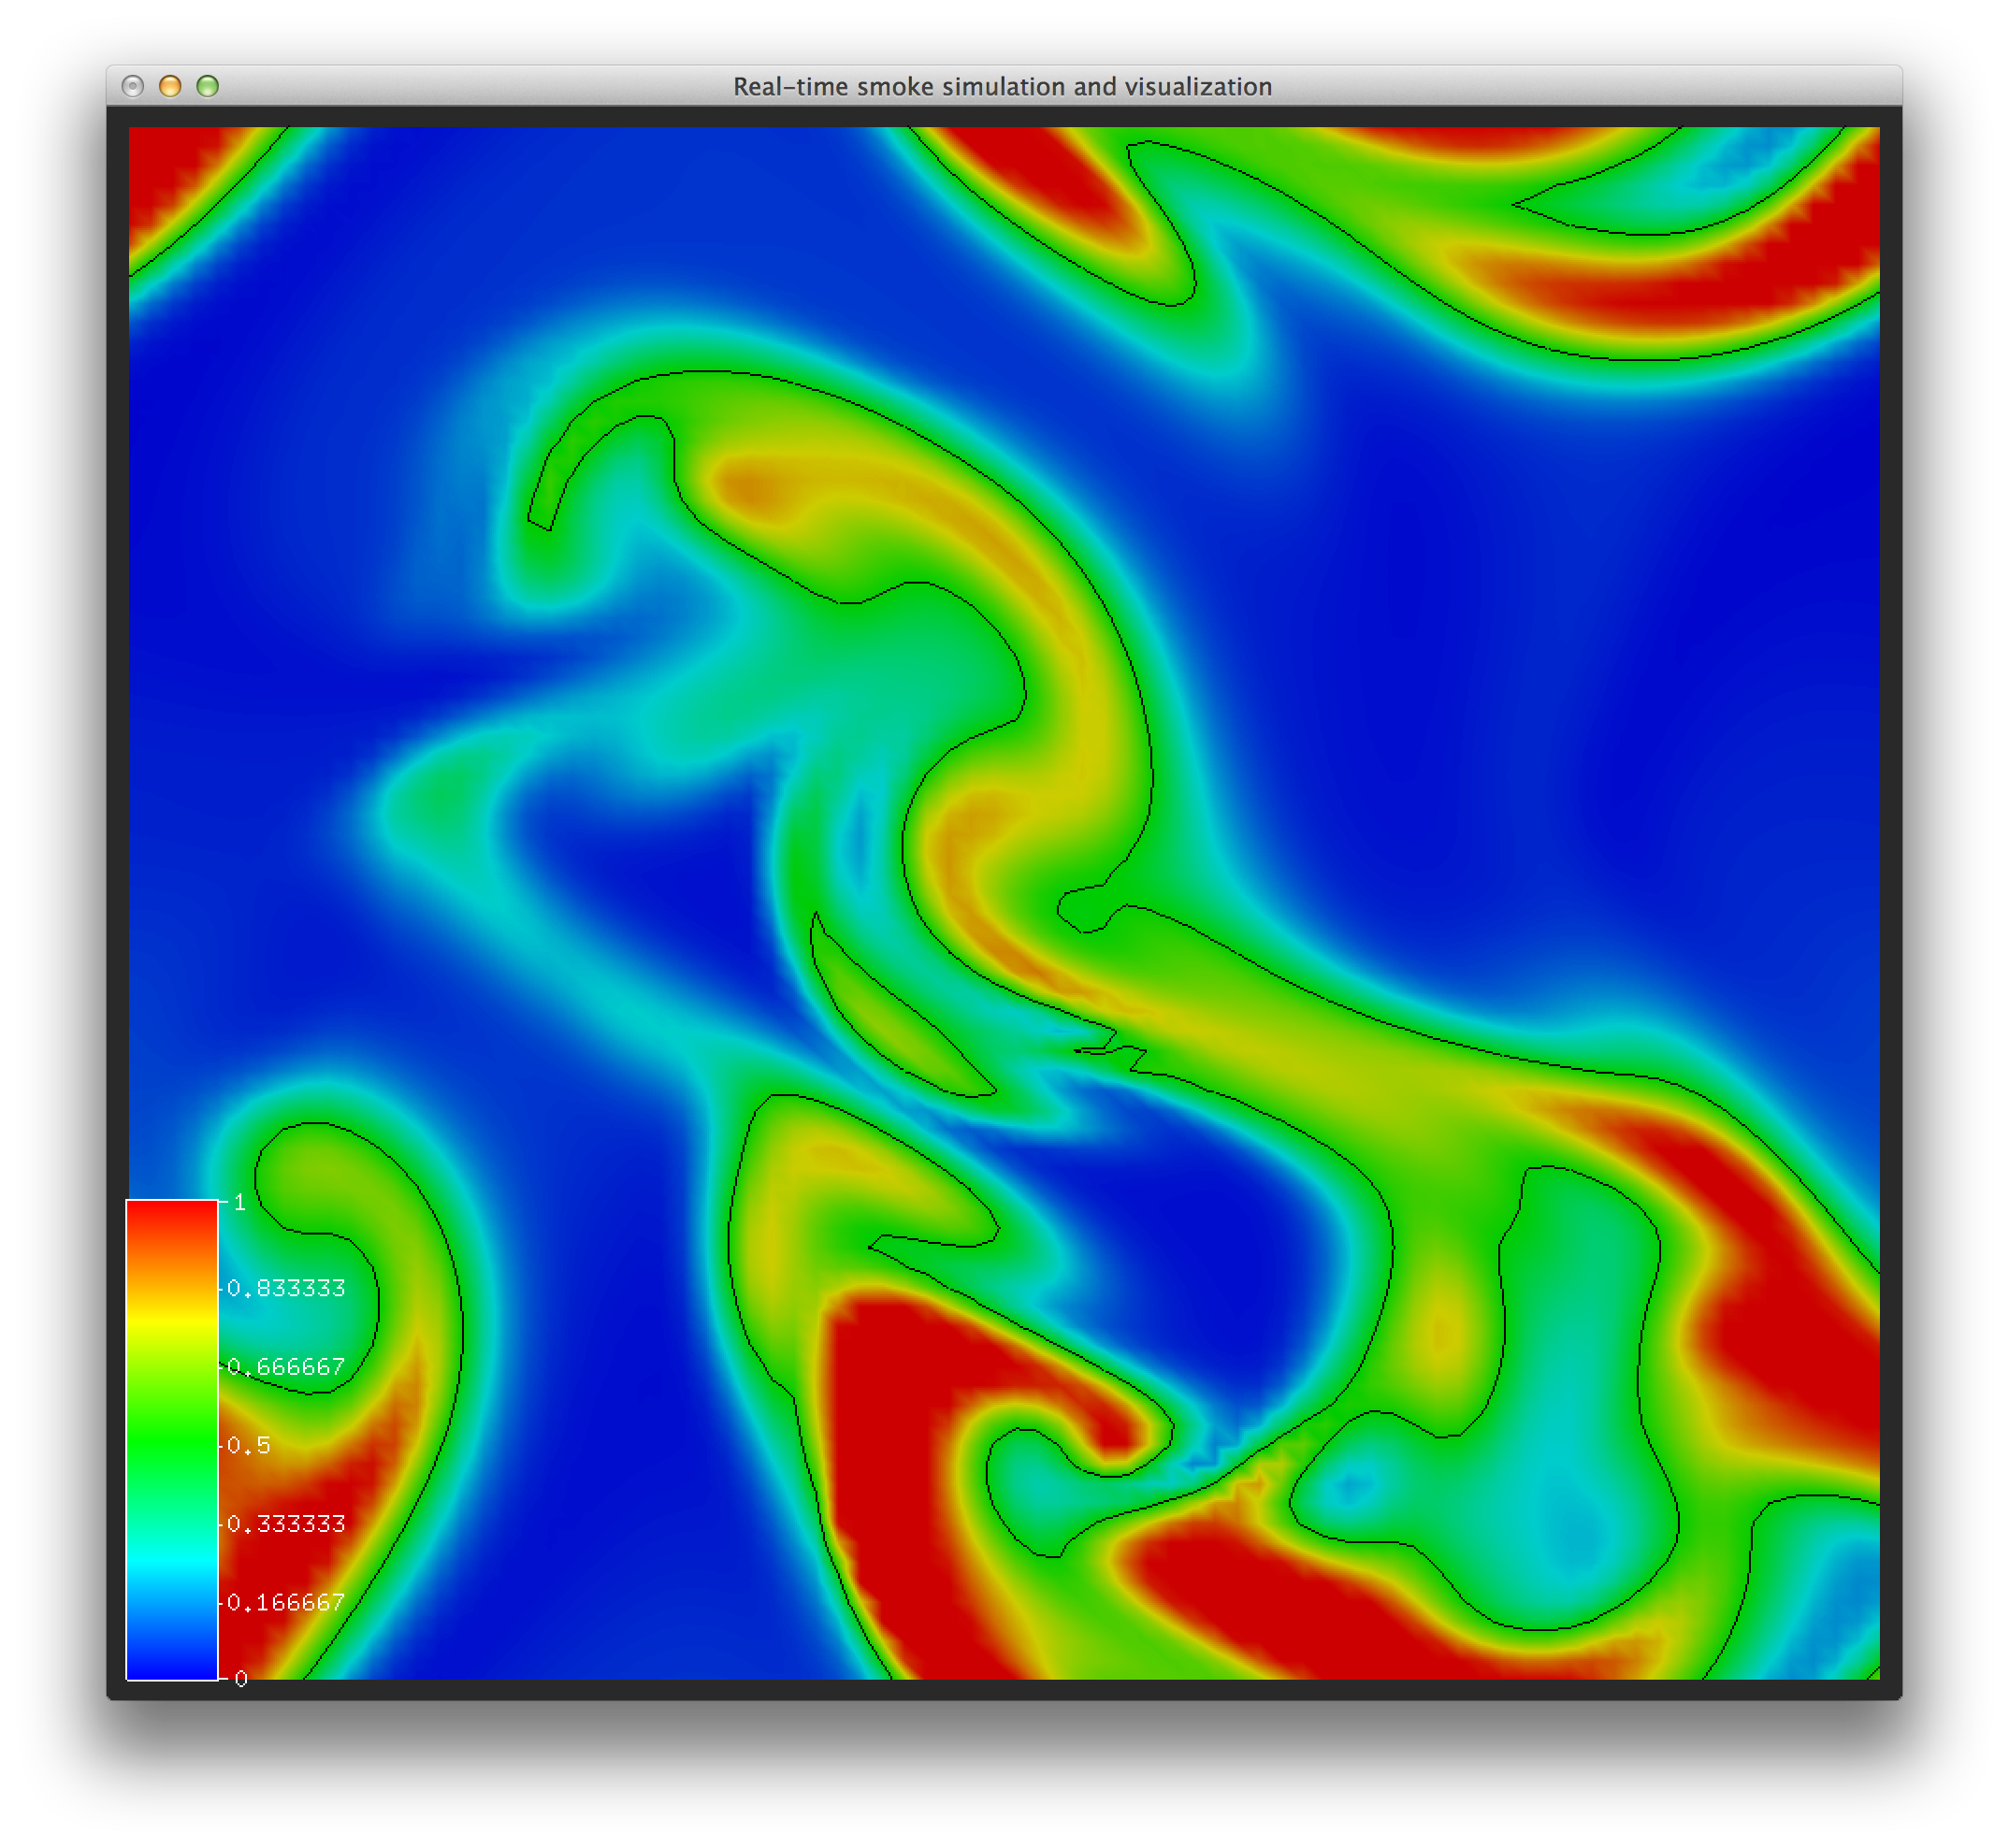
\includegraphics[height=2.7in]{figures/isolines/isolineSmoke.png}
\end{minipage}
\caption{Isolines visualisation of density value $rho = 0.5$. (a) Without smoke visualisation and colorised isolines. (b) With smoke visualisation and not colorised isolines.}
\label{fig:isoline}
\end{center}
\end{figure}

The next kind of isoline visualisation lets the user select a range of density scalar values, \emph{Density rh01} and \emph{Density rho2} respectively, and the number of isolines $N$ to render equally distributed in this range. The number can be set by the control \emph{N Isolines}. Figure~\ref{fig:isolines} shows $N + 1 = 8$ isolines, where $N$ is the number selected by the user, in this case 7, and one more for visualising the isoline with density scalar value $rh0 = 0.5$. The range of the density scalar values is $rho1 = 1.2, rho2 = 0.2$. Listing~\ref{lst:calculateIsolinesScalars} shows the way that the scalar values between the desired range are calculated.

\begin{lstlisting}[language=C++,label=lst:calculateIsolinesScalars,caption={Calculate scalar between range values and draw isolines.}]
float range = fabs(densityRHO2Isoline - densityRHO1Isoline);
float isolineStep = range / numIsolines;

for (int i = 0; i < numIsolines; i++) {
	draw_isoline(simulation, DIM, wn, hn, isolineStep * (i + 1));
}
\end{lstlisting}
 
Figure~\ref{fig:isolines}(a) shows the visualisation of coloured isolines. Figure~\ref{fig:isolines}(b) shows the visualisation of non-colored isolines along with the smoke visualisation. The coloring in both images is done using a rainbow colormap and we have a regularly sampled grid on 80x80. By looking at the images there are some things to be noted. For example, by looking at the top left corner of both images we can identify a spot where many isolines are drawn is a quite tight screen space. This might be undesired taking into consideration the fact that the visualization is not quite clear at this point. This result was produced by selecting to visualize 8 isolines. We can imagine that by selecting to visualize more isolines it could result in cluttering issues.

\begin{figure}[htbp]
\begin{center}
\begin{minipage}[t]{0.48\textwidth}
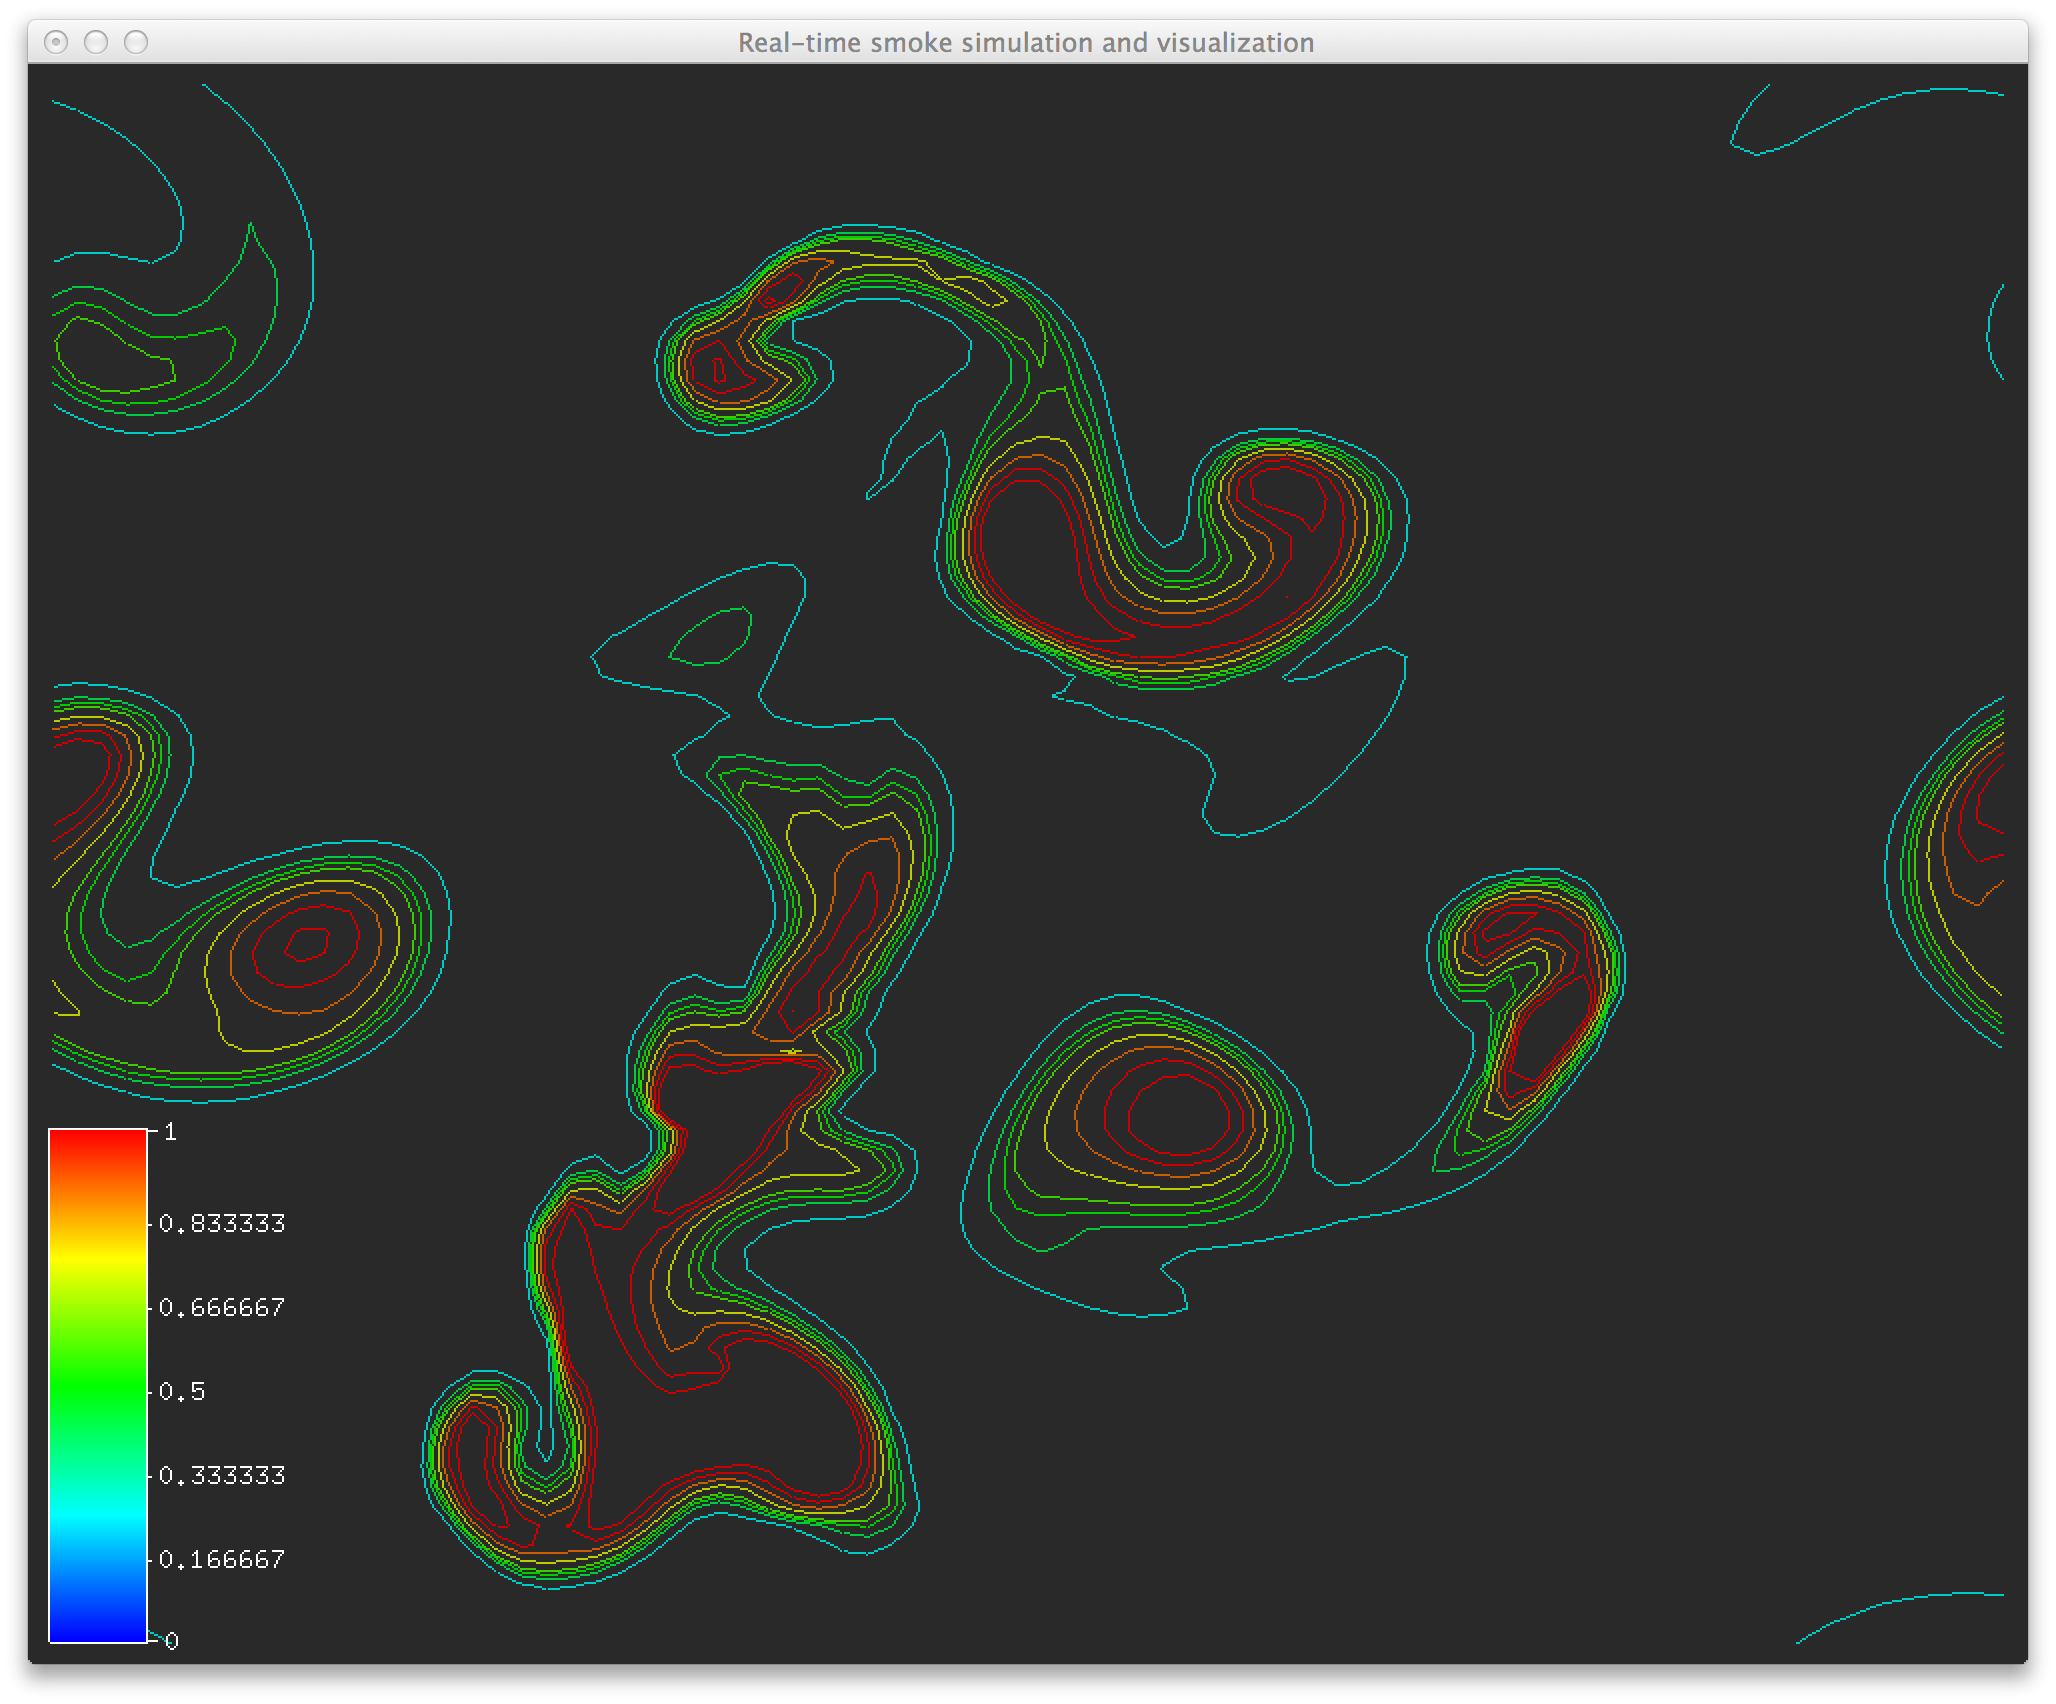
\includegraphics[height=2.5in]{figures/isolines/isolines.png}
\end{minipage}
\begin{minipage}[t]{0.48\textwidth}
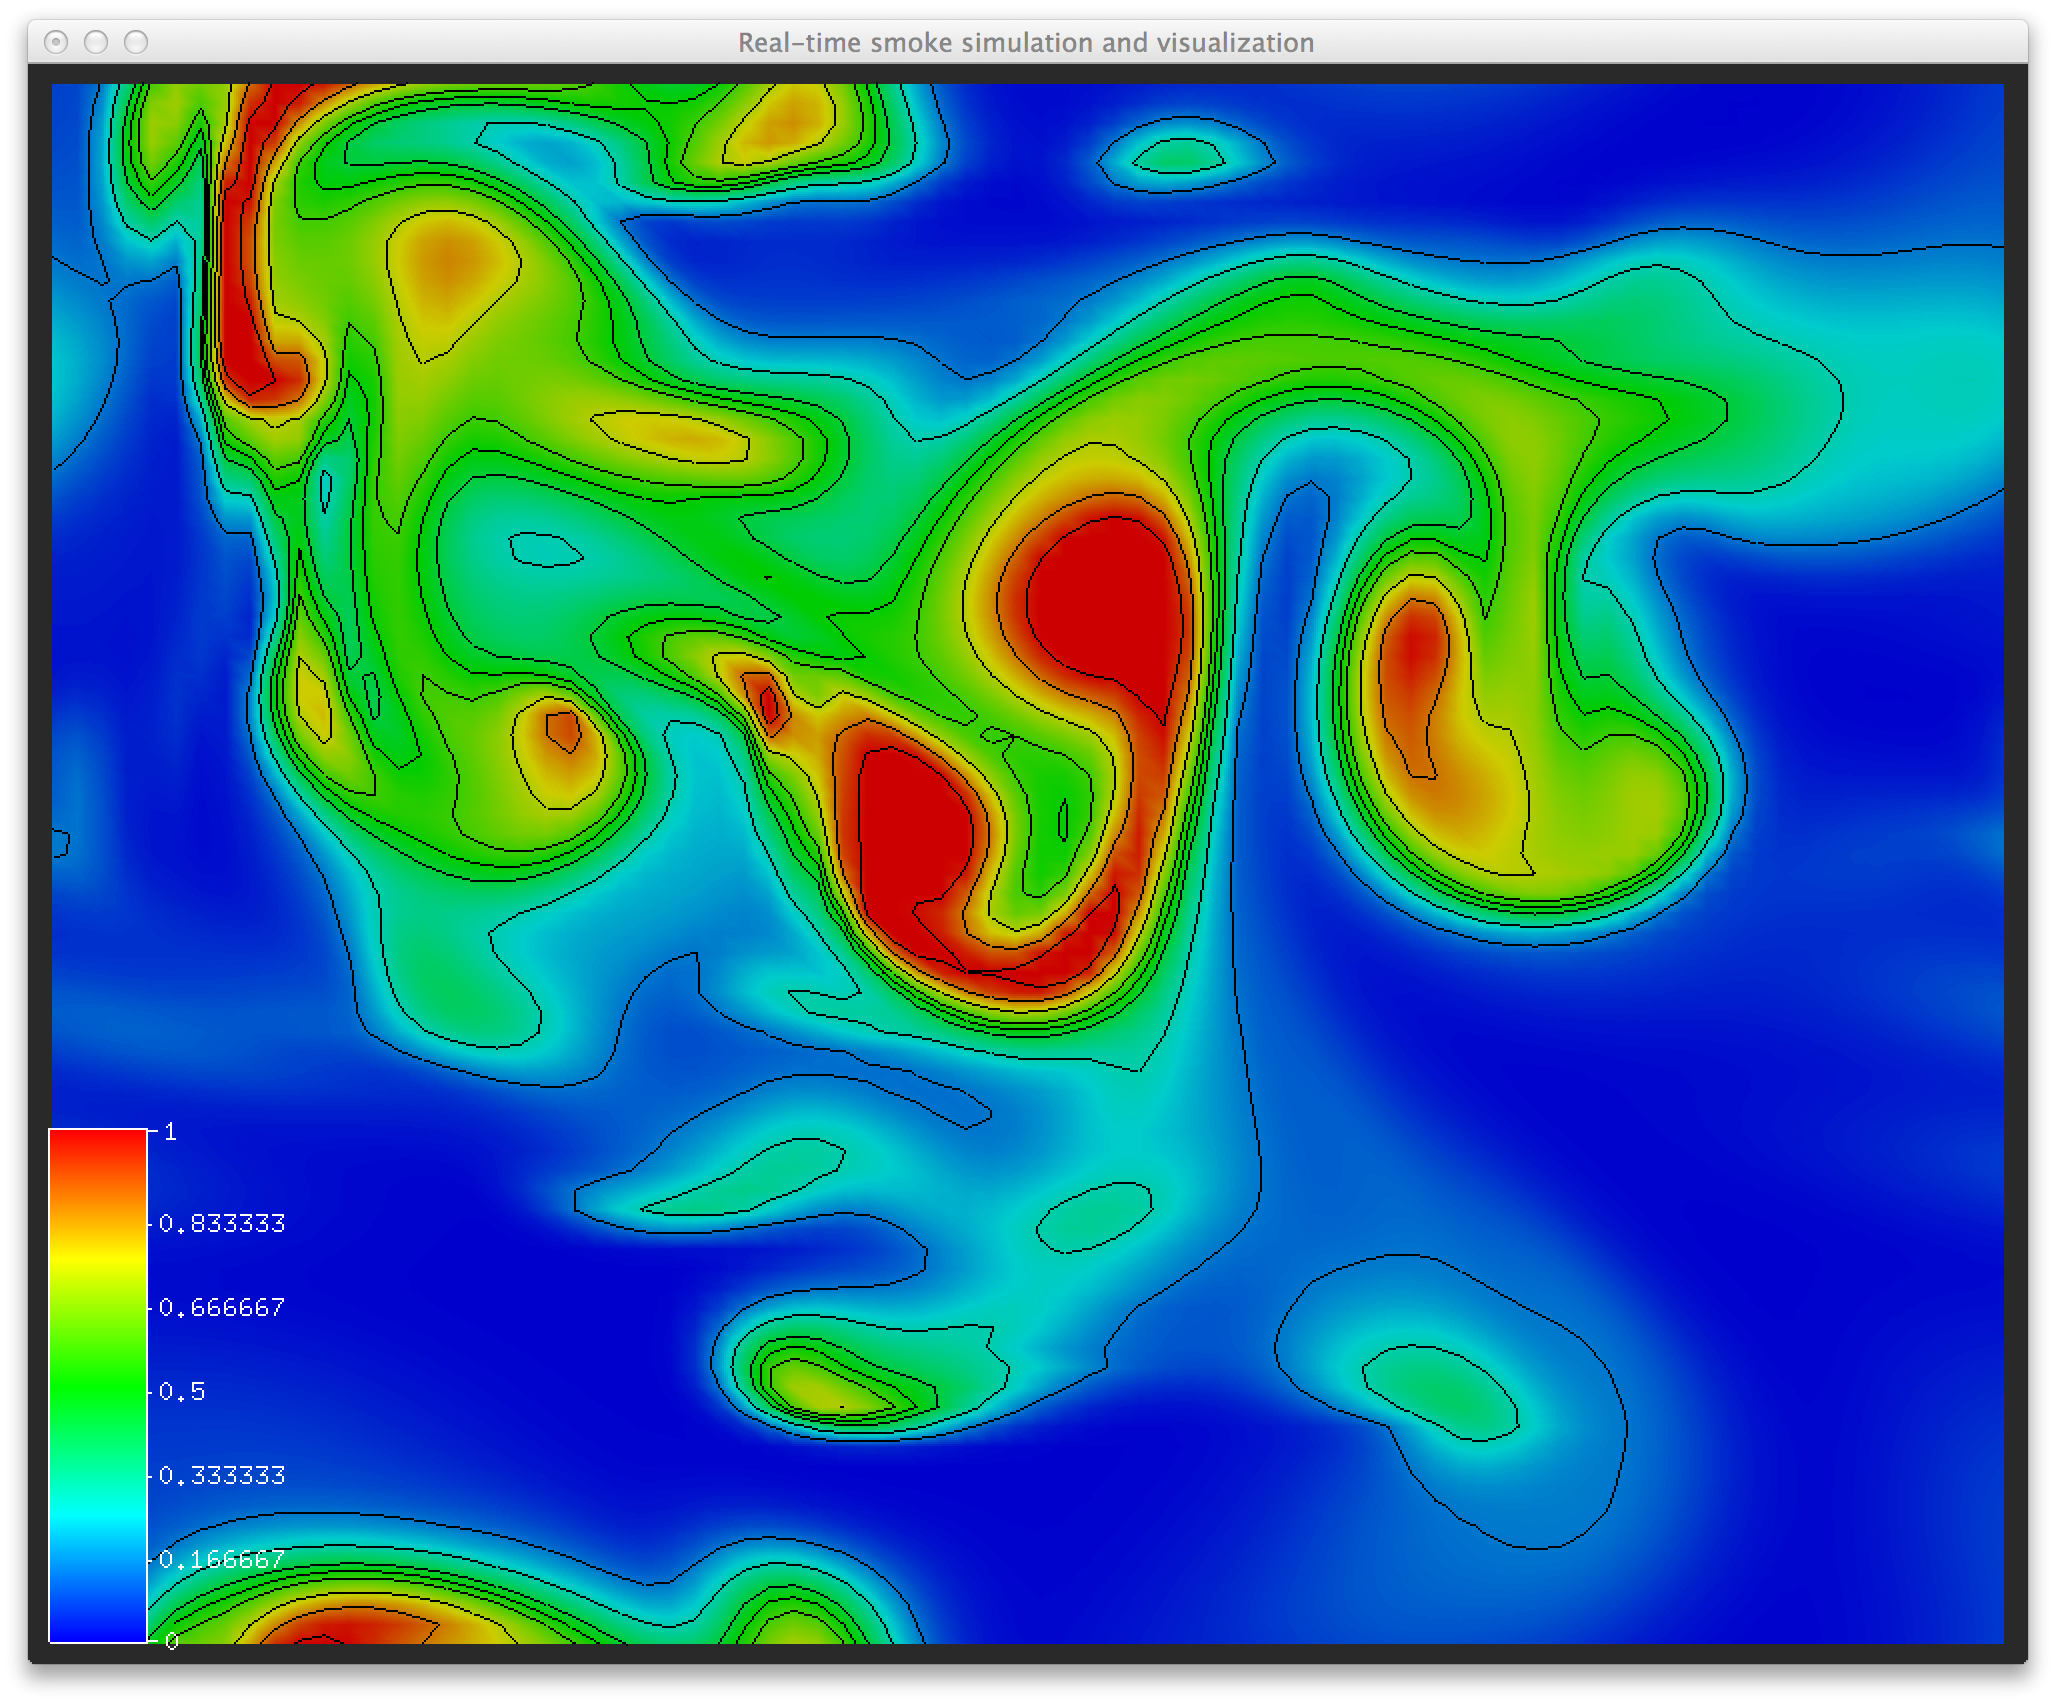
\includegraphics[height=2.5in]{figures/isolines/isolinesSmoke.png}
\end{minipage}
\caption{Isolines visualisation of density value range $rho = 0.5$. (a) Without smoke visualisation and colorised isolines. (b) With smoke visualisation and not colorised isolines.}
\label{fig:isolines}
\end{center}
\end{figure}

Finally, we should note that the visualised isolines (contours) satisfy all the desired properties, such as no intersection, and that they are either closed curves or open curves.